\documentclass[12pt]{article}
\usepackage[a4paper,left=15mm,right=15mm,top=30mm,bottom=20mm]{geometry}

\usepackage{minimal}
\usepackage{xcolor}
\usepackage{listings}
\usepackage{graphicx}
\graphicspath{ {./../artifacts/}}

\DeclareMathOperator{\size}{size}
\DeclareMathOperator{\swap}{swap}
\DeclareMathOperator{\DPLL}{DPLL}
\DeclareMathOperator{\Match}{Matching}


\definecolor{dkgreen}{rgb}{0,0.4,0}
\definecolor{gray}{rgb}{0.5,0.5,0.5}
\definecolor{lightgray}{rgb}{0.96,0.96,0.96}
\definecolor{mauve}{rgb}{0.58,0,0.82}

\def\commentstyle{\color{dkgreen}}
\lstset{ %
  language=C++,                   % the language of the code
  basicstyle=\footnotesize\ttfamily, % the size of the fonts that are used for the code
  numbers=left,                   % where to put the line-numbers
  numberstyle=\footnotesize\color{black},  % the style that is used for the line-numbers
  stepnumber=1,                   % the step between two line-numbers. If it's 1, each line 
                                  % will be numbered
  numbersep=0.7em,                % how far the line-numbers are from the code
  backgroundcolor=\color{lightgray}, % choose the background color. You must add \usepackage{color}
  showspaces=false,               % show spaces adding particular underscores
  showstringspaces=false,         % underline spaces within strings
  showtabs=false,                 % show tabs within strings adding particular underscores
  frame=single,                   % adds a frame around the code
  rulecolor=\color{black},        % if not set, the frame-color may be changed on line-breaks within not-black text (e.g. commens (green here))
  tabsize=2,                      % sets default tabsize to 2 spaces
  breaklines=true,                % sets automatic line breaking
  breakatwhitespace=false,        % sets if automatic breaks should only happen at whitespace
  identifierstyle=\color{blue!25!black},  
  keywordstyle=\color{blue!90!black},      % keyword style
  commentstyle=\commentstyle,     % comment style
  stringstyle=\color{mauve},      % string literal style
  escapeinside={\`}{\`},          % if you want to add a comment within your code
  escapebegin=\commentstyle\footnotesize,
  %morekeywords={n,k},             % if you want to add more keywords to the set
  morecomment=[l][\color{dkgreen}]{\#}, % to color #include<cstdio> 
  morecomment=[s][\commentstyle\color{gray!50!black}]{/**}{*/}
}

\makeindex
\pagestyle{empty}

\title{Методы Оптимизаций\\ Домашнее задание 1 }
\author{Денисов Никита}	

\begin{document}

\maketitle

\section{Эксперимент: Траектория градиентного спуска на
квадратичной функции} % 1

Взял 3 квадратичные функции для экспериментов.

\begin{enumerate}


\item % 1

$$
A = 
\begin{pmatrix}
1 & 2 \\
2 & 5
\end{pmatrix},
\
b = 
\begin{pmatrix}
0 \\
0
\end{pmatrix}
$$

\item % 2

$$
A = 
\begin{pmatrix}
1 & 1 \\
1 & 10
\end{pmatrix},
\
b = 
\begin{pmatrix}
1 \\
1
\end{pmatrix}
$$

\item % 3

$$
A = 
\begin{pmatrix}
5 & 1 \\
1 & 5
\end{pmatrix},
\
b = 
\begin{pmatrix}
4 \\
1
\end{pmatrix}
$$

\end{enumerate}

Попробовал разные стратегии шага для каждой функции с фиксированной начальной точкой

\begin{enumerate}

\item % 1

$$
x_0 = 
\begin{pmatrix}
10 \\
1.5
\end{pmatrix}
$$

Armijo
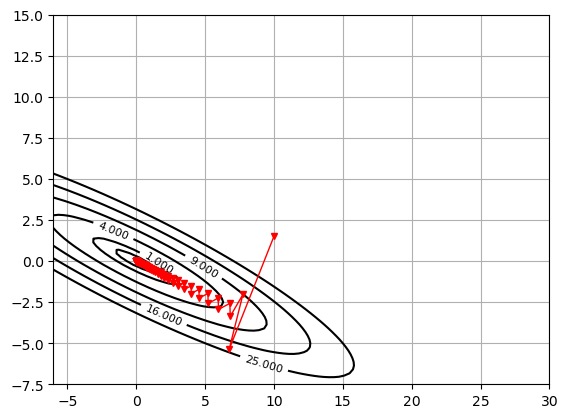
\includegraphics{exp1/strategies/1_armijo.png}


Wolfe
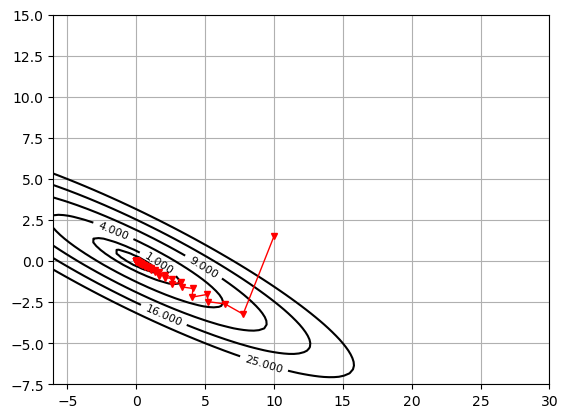
\includegraphics{exp1/strategies/1_wolfe.png}


Constant
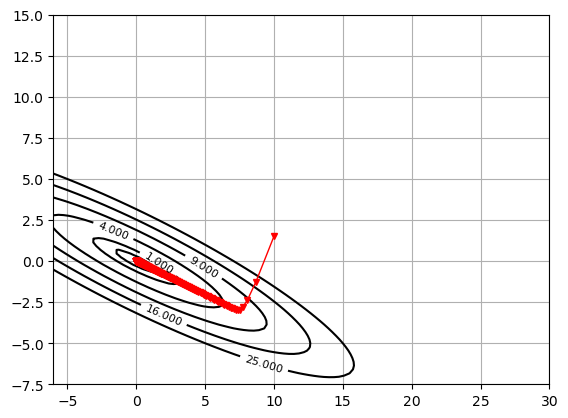
\includegraphics{exp1/strategies/1_constant.png}

\item % 2

$$
x_0 = 
\begin{pmatrix}
25 \\
5.5
\end{pmatrix}
$$

Armijo
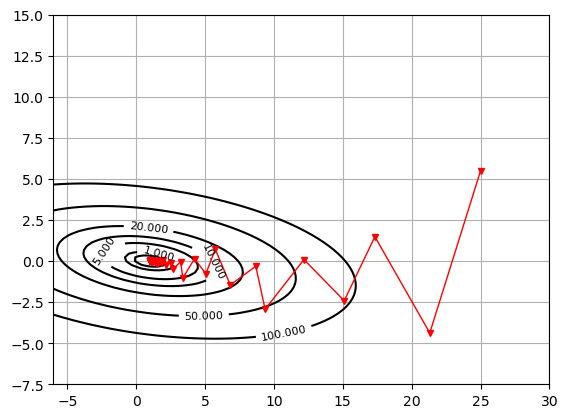
\includegraphics{exp1/strategies/2_armijo.png}


Wolfe
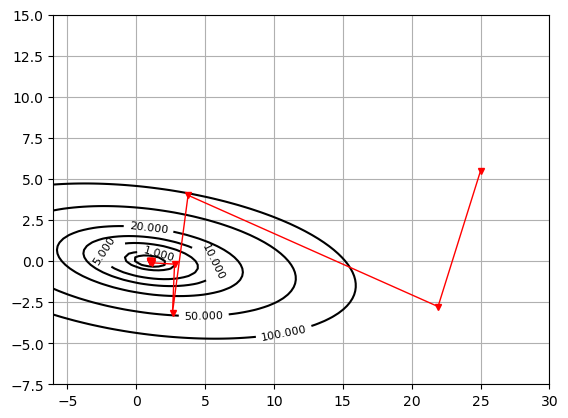
\includegraphics{exp1/strategies/2_wolfe.png}


Constant
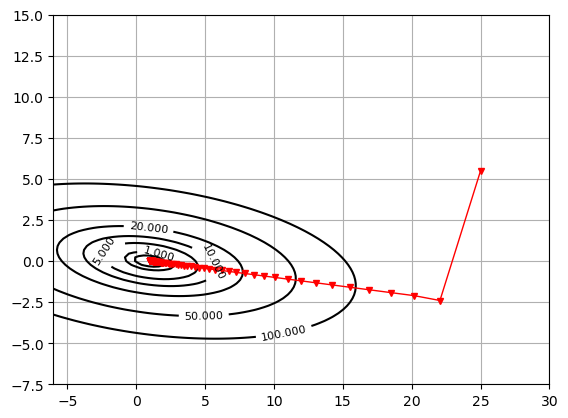
\includegraphics{exp1/strategies/2_constant.png}

\item % 3

$$
x_0 = 
\begin{pmatrix}
5 \\
15.5
\end{pmatrix}
$$

Armijo
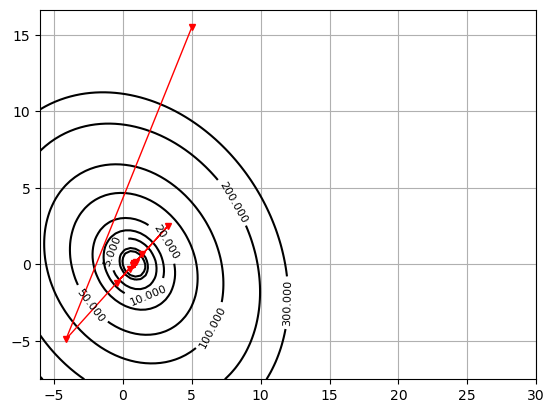
\includegraphics{exp1/strategies/3_armijo.png}


Wolfe
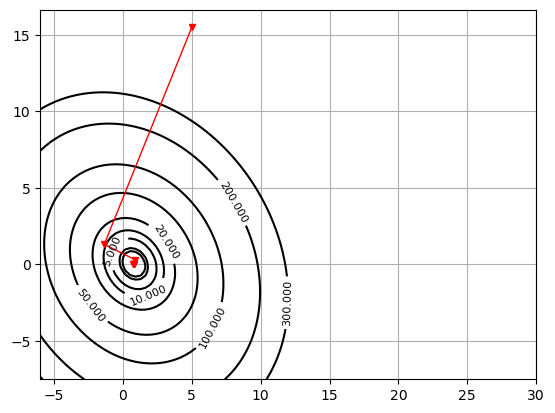
\includegraphics{exp1/strategies/3_wolfe.png}


Constant
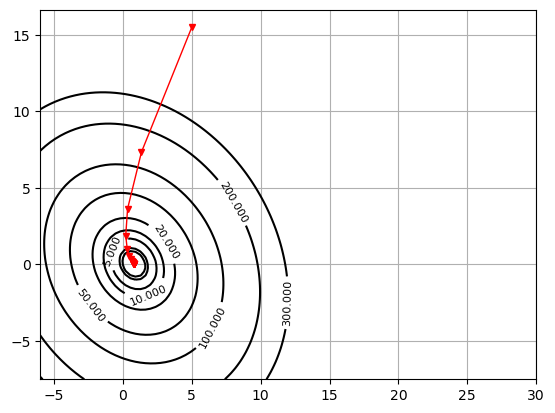
\includegraphics{exp1/strategies/3_constant.png}


\end{enumerate}


Далее взял вторую функцию и несколько различных начальных точек

\begin{enumerate}

\item % 1

$$
x_0 = 
\begin{pmatrix}
25 \\
5.5
\end{pmatrix}
$$

Armijo
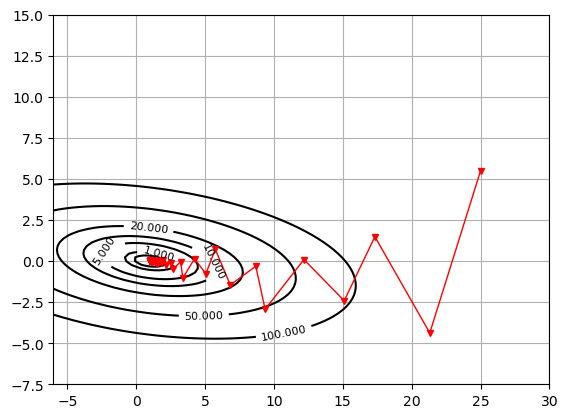
\includegraphics{exp1/x_0/1_armijo.png}


Wolfe
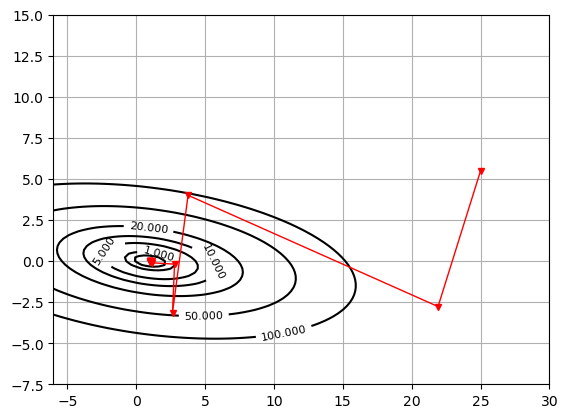
\includegraphics{exp1/x_0/1_wolfe.png}


Constant
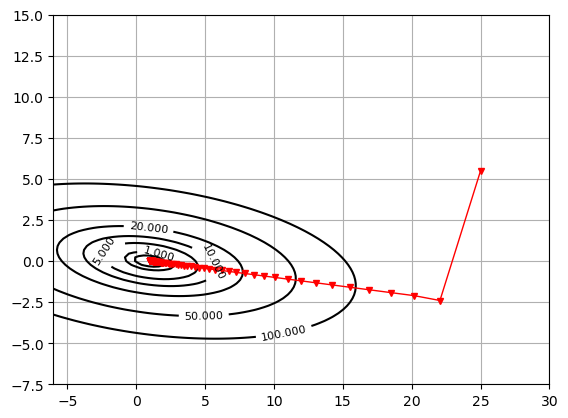
\includegraphics{exp1/x_0/1_constant.png}

\item % 2

$$
x_0 = 
\begin{pmatrix}
5 \\
5
\end{pmatrix}
$$

Armijo
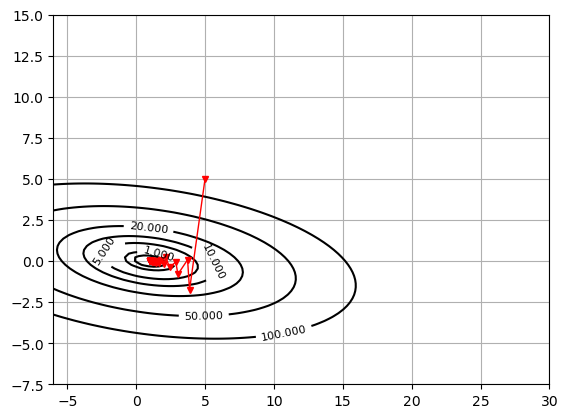
\includegraphics{exp1/x_0/2_armijo.png}


Wolfe
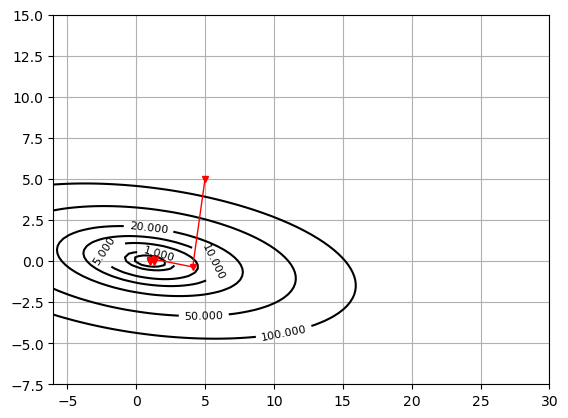
\includegraphics{exp1/x_0/2_wolfe.png}


Constant
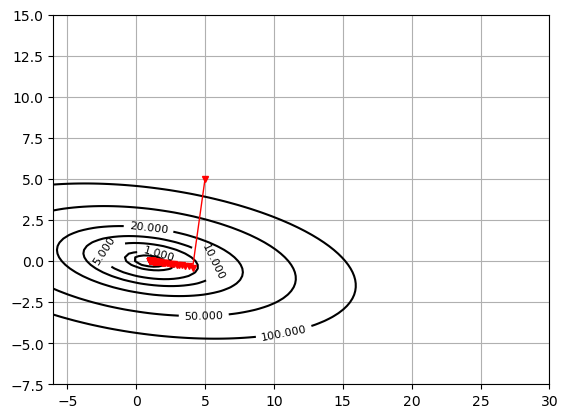
\includegraphics{exp1/x_0/2_constant.png}

\item % 3

$$
x_0 = 
\begin{pmatrix}
25 \\
-3
\end{pmatrix}
$$

Armijo
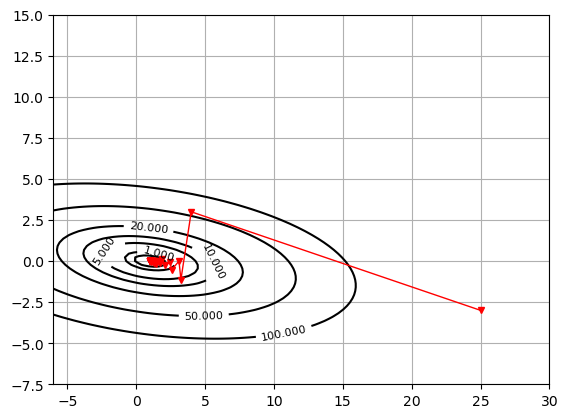
\includegraphics{exp1/x_0/3_armijo.png}


Wolfe
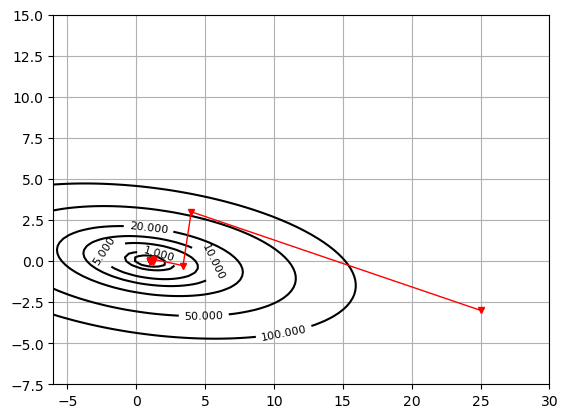
\includegraphics{exp1/x_0/3_wolfe.png}


Constant
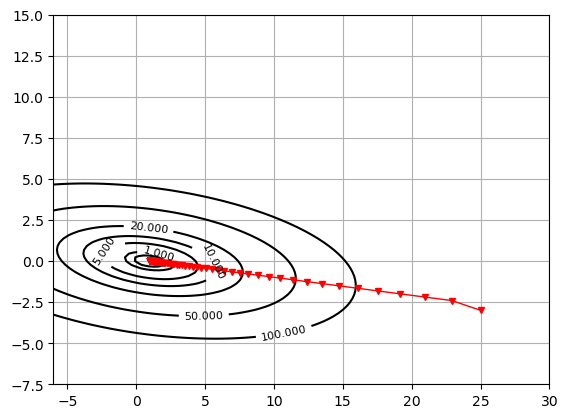
\includegraphics{exp1/x_0/3_constant.png}


\end{enumerate}

Вывод по этому эксперименту:

Поведение метода градиентного спуска действительно отличается в зависимости от метода и от начальной точки для разных начальных функций.  Так, для константной стратегии при небольшом шаге происходит больше итераций для сходимости, чем для Армихо и Вульфа. При этом линия сходимости получается плавная по линиям уровня. Армихо шагает быстрее, но перепрыгивает и колеблется вокруг линии (проходящей так, что линии уровня разбиваются симметрично). Вульф сходится еще быстрее Армихо (так как хорош для квадратичных функций). Начальная точка в основном влияет на скорость сходимости: чем ближе она расположена к оптимуму и чем удачнее попадется на линии уровня, тем быстрее сойдется.

\section{Эксперимент: Зависимость числа итераций градиентного спуска от числа обусловленности и размерности пространства} % 2

\end{document}
